%% tex/NPClass.tex
%% Copyright 2019 Andrea Berlingieri
%
% This work may be distributed and/or modified under the
% conditions of the LaTeX Project Public License, either version 1.3
% of this license or (at your option) any later version.
% The latest version of this license is in
%   http://www.latex-project.org/lppl.txt
% and version 1.3 or later is part of all distributions of LaTeX
% version 2005/12/01 or later.
%
% This work has the LPPL maintenance status `maintained'.
%
% The Current Maintainer of this work is Andrea Berlingieri.
%
% This work consists of all files listed in manifest.txt
\chapter{La classe $\NPClass$}

%Slide 105
Vediamo ora due argomenti importanti concentrando la nostra attenzione su una classe di complessita'
molto interessante: $\NPClass$. I due argomenti che trattiamo sono il teorema della proiezione e la
nozione di riducibilita'.

\section{Teorema della proiezione}

Il teorema della proiezione e' importante perche' mette in relazione le due visioni della classe
$\NPClass$: una, che la definisce, e' quella di insieme dei linguaggi riconoscibili da una macchina
non deterministica, e l'altra, interessante a livello pratico, e' quella di insieme dei problemi per
cui esistono algoritmi di verifica della soluzione che operano in tempo polinomiale.

\begin{thm}
    \textbf{(Teorema della proiezione).} Dato un linguaggio $A \subseteq \Sigma^{*}$, $A \in
    \NPClass$ se e solo se esiste un linguaggio $B \in \PClass$ e un polinomio $p$ tale che per ogni
    $x \in \Sigma^{*}$
    \begin{equation*}
        x \in A \iff \exists y, |y| \leq p(|x|) \land \pair{x}{y} \in B
    \end{equation*}
\end{thm}

$y$ e' un certificato che dipende da $x$. E' un'informazione aggiuntiva rispetto ad $x$ che ci
permette di fare una verifica veloce. E' una sorta di ``prova'' che $x$ appartiene in effetti al
linguaggio $A$. L'utilita' di $B$ sta nel fatto che ci permette di verificare in tempo polinomiale
l'autenticita' del certificato per $x$.

Che cosa sia il cerficicato non e' ben definito: dipende dal problema e sta a noi definire cosa sia
un buon cerificato. Dato che noi consideriamo solo problemi decisionali il certificato puo' essere
qualunque informazione che ci permetta di verificare che la risposta sia ``Si'''.

Chiediamo inoltre che la dimensione del certificato non cresca esponenzialmente. Il motivo e' che
input grandi ci danno complessita' basse che sono tuttavia fittizie, un po' come accadeva per il
padding.

Ad esempio per il problema della tautologia abbiamo un algoritmo lineare nella dimensione di una
tabella di verita' che verifica se la tabella e' ben formata, e quindi se una formula data e'
tautologica. Tuttavia questa tabella ha dimensione esponenziale. L'algoritmo risulta efficiente se
confrontato con la dimensione della tabella, ma risulta pessimo se confrontato con la dimensione del
nostro input, ovvero la formula di partenza. Di conseguenza non si tratta di un buon certificato per
noi.

\begin{proof}

    Sia $A \subseteq \Sigma^{*}$, $A \in \NPClass$ e sia $x$ una stringa in $A$. Abbiamo che $A \in
    \NPClass$ sse esiste una MdTN $M$ che riconosce $A$. Che certificato possiamo dare per $x$?
    Come certificato possiamo prendere la sequenza delle scelte prese da $M$ in una computazione che
    riconosce $x$, insieme a $\code{M}$. Quanto e' grande questa sequenza? E' polinomiale in $|x|$,
    essendo $A \in \NPClass$. Esiste quindi un cammino accettante polinomiale nel numero di passi.
    Il codice di $M$ e' costante nella sua dimensione e non influisce a livello della complessita'.
    Sia $B$ il linguaggio delle coppie $x$-certificato. Dato $x$ ed il suo certificato una macchina
    deterministica $M'$ che riconosce il linguaggio $B$ effettua una simulazione di $M$ usando le scelte
    fornite. Se la configurazione finale della simulazione di $M$ e' accettante la machina $M'$
    accetta la coppia $x$-certificato; in caso contrario rifiuta. E' facile verificare il secondo $\iff$
    dell'enunciato del teorema data questa definizione di $M'$ e $B$. Inoltre abbiamo che $B \in
    \PClass$, dato che l'estrazione del certificato dalla coppia e' un'operazione con complessita'
    lineare rispetto alla dimensione di questa e la simulazione di $M$ richiede un numero di passi
    polinomiale in $|x|$.

    Viceversa supponiamo ora di avere $B \in \PClass$. Vogliamo dimostrare che se prendiamo un
    polinomio $p$ e facciamo la proiezione esistenziale bound da $p$ abbiamo che il linguaggio
    ottenuto in questo modo sta in $\NPClass$. In particolare vogliamo dimostrare che il linguaggio
    \begin{equation*}
        A = \set{x \mid \exists y, y \leq p(|x|) \land \pair{x}{y} \in B}
    \end{equation*}
    fa parte di $\NPClass$.

    Per mostrare cio' esibiamo una MdTN $M$ che ci permetta di riconoscere $A$. $M$ funziona nel
    seguente modo: dato $x$ genera tutti i certificati $y$ di dimensione minore o uguale a $p(|x|)$
    e testa l'appartenenza di $\pair{x}{y}$ a $B$ in tempo polinomiale per tutti. Se uno di questi
    certificati risulta valido $M$ accetta $x$, altrimenti rifiuta. La quantita' di certificati da
    testare e' esponenziale, dato che il numero di certificati diversi di lunghezza $p(|x|)$ e'
    $|\Sigma|^{p(|x|)}$. Sfruttando il fatto che la macchina deterministica e' ``fortunata''
    generiamo non deterministicamente il certificato corretto per $x$. $M$ riconosce quindi $x
    \in A$ in tempo polinomiale non deterministico.

\end{proof}

Non e' restrittivo supporre, come abbiamo fatto implicitamente, che $B$ sia un linguaggio sullo
stesso alfabeto $\Sigma$ di $A$.

\section{Riducibilita'}

%Slide 112

La nozione di riducibilita' che vediamo e' molto simile a quella della teoria della complessita'.

\begin{defn}
    Siano $A,B \in \Sigma^{*}$ due linguaggi. Diremo che $A$ e' riducibile in tempo polinomiale a
    $B$, $A \leq_{p} B$, se esiste $f \in \FP$ tale che per ogni $x \in \Sigma^{*}$, $x \in A \iff
    f(x) \in B$.
\end{defn}
Se al vincolo polinomiale alla complessita' di $f$ andiamo a sostituire un diverso vincolo sulla
complessita' in tempo o in spazio otteniamo una nozione di riducibilita' analoga a questa ma diversa
nel numero e nella natura delle riduzioni.

La nozione di riducibilita' e' many-to-one. Vogliamo che $f$ sia calcolabile in tempo polinomiale.
Nella definizione di riducibilita' dobbiamo fare attenzione ad un dettaglio tecnico.  Dire che $f
\in \PClass$ e' sbagliato perche' $f$ non e' un linguaggio, bensi' una funzione. Per questo motivo
introduciamo $\FP$ come l'insieme delle funzioni calcolabili in tempo polinomiale, ovvero delle $f$
per le quali esiste una MdT che calcola $f$ in tempo polinomiale.

Qualunque tipo di nozione di riducibilita' e' ragionevole. Piu' sono deboli i vincoli che poniamo
alla complessita' di $f$ piu' la nostra nozione di riduzione sara' lasca e maggiori saranno le
riduzioni possibili. Intuitivamente se disponiamo di un numero elevato di risorse e' piu' facile
ridurre un linguaggio ad un altro, mentre se le risorse disponibili sono limitate le riduzioni
possibili diminuiscono. Ad esempio una riducibilita' esponenziale permetterebbe di ridurre molti
problemi tra loro. Noi ci concentriamo unicamente sulla riducibilita' polinomiale in tempo. E'
generalmente la piu' interessante.

Le riducibilita' sono in genere dei preordini. Ricordiamo che un preordine e' una relazione binaria
riflessiva e transitiva. Per la riducibilita' polinomiale in tempo la proprieta' riflessiva e'
dimostrabile in maniera ovvia. Per la transitivita' supponiamo di avere $A,B,C$ con $A \leq_{p} B$
attraverso $f$ e $B \leq_{p} C$ attraverso $g$. Ci basta comporre $f$ e $g$ per ottenere $h$
calcolabile con complessita' polinomiale che riduce $A$ a $C$. Questa composizione ha complessita'
polinomiale perche' la composizione di polinomi e' ancora un polinomio. Questo vale anche per
$\leq_{L}$, la riducibilita' in $\LOGSPACE$.

%Slide 113

\begin{defn}
    Sia $\CClass$ una classe di linguaggi e sia $\leq$ un qualche preordine. Diremo che $\CClass$ e'
    chiusa rispetto a $\leq$ se
    \begin{equation*}
        A \leq B \land B \in \CClass \implies A \in \CClass
    \end{equation*}
\end{defn}

Si puo' dimostrare che che $\PClass$, $\NPClass$ e $\PSPACE$ sono chiuse rispetto alla riduzione
polinomiale.

Supponiamo infatti di avere due linguaggi $A$ e $B$, con $B \in \PClass$, e di voler riconoscere il
linguaggio $A$. Sia $x$ la stringa che vogliamo riconoscere. Se esiste una funzione di riduzione $f
\in \FP$ da $A$ a $B$ possiamo calcolare la riduzione $f(x)$ in tempo polinomiale.  Sappiamo che la
dimensione di $f(x)$ sara' polinomiale rispetto alla dimensione di $x$, dato che $f$ e' stata
calcolata in tempo polinomiale e lo spazio e' bound dal tempo. Inoltre verificare che $f(x) \in B$
richiede tempo polinomiale. Poiche' la composizione di polinomi rimane un polinomio questa procedura
di riconoscimento di $A$ ha complessita' polinomiale. Lo stesso discorso si applica se al posto di
$\PClass$ abbiamo $\NPClass$.

Una classe come $\LOGSPACE$ non e' chiusa rispetto alla riducibilita' in tempo polinomiale. E'
chiusa rispetto alla riducbilita' in spazio logaritmico. Supponiamo che $B \in \LOGSPACE$ e che $A
\leq_{p} B$. Questo non implica che $A \in \LOGSPACE$. Gia' il valore di $f(x)$ puo' avere
dimensione polinomiale, e lo spazio logaritmico non ci basta. Il problema e' che questa nozione di
riducibilita' e' troppo lasca per la classe che vogliamo studiare e ne serve una piu' precisa.

La classe $\PClass$ non e' chiusa rispetto alla riduzione esponenziale. Infatti possiamo ridurre un
qualsiasi problema $A$ in tempo esponenziale ad uno piu' semplice $B \in \PClass$. Questo non
implica che abbiamo un algoritmo per risolvere $A$ in tempo polinomiale e che quindi $A \in
\PClass$.

Vedremo che tutti i problemi non banali in $\PClass$ sono mutuamente riducibili con una riduzione
polinomiale. Inoltre tutti i problemi in $\EXP$ sono $\EXP$-completi. Infine esiste una riduzione
esponenziale da un problema in $\EXP$ ad uno in $\PClass$.

%Slide 114

\section{$\NPClass$-completezza e $\NPClass$-hardness}

La definizione di problema arduo e problema completo puo' essere data per qualsiasi classe di
complessita'. Noi siamo interessati a $\NPClass$.

\begin{defn}
    Sia $\CClass$ una classe di linguaggi e $\leq$ un preordine tra di essi. Sia $B$ un linguaggio.
    Abbiamo che
    \begin{itemize}
        \item $B$ e $\CClass$-arduo rispetto a $\leq$ se ogni $A \in \CClass$ e' riducibile a $B$;
        \item $B$ e $\CClass$-completo rispetto a $\leq$ se $B \in \CClass$ e $B$ e' $\CClass$-arduo;
    \end{itemize}
\end{defn}

Un problema $\CClass$-arduo e' il problema piu' complicato della classe. Questa nozione di
complicatezza pero' dipende dalla quantita' di risorse che diamo alla nozione di riducibilita.  Meno
risorse diamo alla funzione di riduzione, meno sono le riduzioni possibili, e piu' fini sono le
distinzioni tra classi, e analogamente con piu' risorse vale il contrario.

\begin{defn}
    Sia $B$ un linguaggio. Diciamo che $B$ e' $\NPClass$-hard se $\forall A \in \NPClass, A \leq_{p}
    B$. Diciamo che $B$ e' $\NPClass$-completo se $B$ e' $\NPClass$-hard e inoltre $B \in \NPClass$.
\end{defn}

I problemi $\NPClass$-completi sono quei problemi a cui tutti gli altri sono riducibili. Se avessimo
un modo efficiente per risolvere un problema $\NPClass$-completo $A$ sapremmo che, per ogni altro
problema in $\NPClass$, esisterebbe un algoritmo efficiente di soluzione che utilizza una riduzione
polinomiale dal problema da risolvere ad $A$ e l'algoritmo per $A$.

L'$\NPClass$-completezza e' interessante a livello pratico. Un problema che sappiamo essere
$\NPClass$-completo e' $\SAT$. Esistono algoritmi molto efficienti che possono risolvere $\SAT$ in
maniera efficiente nonostante la loro complessita' nel caso pessimo rimanga esponenziale. Si
utilizzano proprieta' di sottoclassi particolari di formule proposizionali che permettono di avere
algoritmi di soluzione generalmente efficienti. Non e' una cattiva idea risolvere un problema
trovando una riduzione polinomiale a $\SAT$ e usare un $\SAT$-solver, dato che $\SAT$ e' stato molto
investigato ed esistono algoritmi ed euristiche efficienti. Si potrebbe fare la stessa cosa
utilizzando altri problemi $\NPClass$-completi.

Non si sa se tutti i problemi in $\NPClass$ sono $\NPClass$-completi. Per $\PClass$ questa cosa
invece vale.  Se riusciamo a dimostrare che esiste un problema in $\NPClass$ non $\NPClass$-completo
abbiamo come conseguenza che
$\PClass \not= \NPClass$.

%Uguaglianza di Leibniz: $x = y \iff \forall P, P(x) \iff P(y)$. Due oggetti sono uguali se qualsiasi
%osservazione facciamo su di essi otteniamo lo stesso risultato. Se dimostriamo che c'e' qualche
%proprieta' che vale per un $x$ ma non per un $y$ abbiamo che $x \not= y$.

La questione $\PClass$ vs $\NPClass$, ovvero determinare se queste due classi coincidono o sono
diverse, e' uno dei Millenium Problems. C'e' in palio un premio di 1 milione di dollari per chi
fosse in grado di risolvere questo problema, o fare comunque passi importanti verso la risoluzione.
Si congettura che $\PClass \not= \NPClass$.

Una problematica ancora aperta e altrettanto interessante e' la dimostrazione che l'inclusione tra
$\PClass$ e $\PSPACE$ e' stretta. $\PSPACE$ e' una classe molto grande, che contiene anche
$\NPClass$, e molto distante da $\PClass$. Si congettura che l'inclusione sia stretta, ma non si e'
ancora riusciti a dimostrarlo. Un problema con questa dimostrazione e' legato al fatto che le due
classi sono definite da risorse diverse. Lavorare con risorse diverse a livello di complessita' e'
sempre delicato e non banale.

%Slide 116

Vediamo un esempio di problema $\NPClass$-completo

Dimostrare la completezza di un problema non e' ovvio. Infatti dobbiamo dimostrare che tutti i
problemi in $\NPClass$ sono riducibili al problema che vogliamo dimostrare essere completo.

Il problema che consideriamo e' il problema limitato della fermata con macchine non deterministiche.

\begin{thm}
    Sia $\BHP$ il linguaggio cosi' definito:
    \begin{equation*}
        \BHP = \set {\tuple{x,y,0^{t}} \mid \text{La MdTN $M$ accetta $y$ in tempo
        $\textit{time}_{M_{x}}(y) \leq t$}}
    \end{equation*}
    $\BHP$ e' $\NPClass$-completo
\end{thm}

Il tempo e' dato in formato unario. Di solito si fa cosi' quando vogliamo una complessita' lineare
in un dato tempo.  Se dessimo una rappresentazione logaritmica del tempo l'algoritmo che lavora con
quel tempo risulterebbe avere complessita' esponenziale.

\begin{proof}
    La prima cosa da fare e' dimostrare che questo problema sta in $\NPClass$. Costruiamo una MdTN
    $M$ che riconosce $\BHP$. $M$ opera nel seguente modo: verifica innanzitutto che la stringa in
    input sia una tripla la cui prima componente sia il codice di una MdTN. Dopodiche' simula la
    computazione della macchina $M_{x}$ su input $y$ con bound dato da $t$. Ad ogni scelta non
    deterministica di $M_{x}$ corrisponde una scelta non deterministica di $M$. Se alla fine della
    simulazione abbiamo che $M_{x}$ riconosce $y$ abbiamo che $M$ accetta, altrimenti rifiuta.
    Rifiuta inoltre se la simulazione supera il bound in tempo.

    Supponiamo ora di avere un linguaggio $A \in \NPClass$ e di volerlo riconoscere, ovvero decidere
    $y \in A$.  Possiamo farlo con una riduzione polinomiale a $\BHP$: prendiamo il codice $x$ di
    una MdTN $M$ che riconosce $A$ in tempo polinomiale, l'input $y$ da riconoscere e come tempo $t$
    prendiamo $p(|y|)$, dove $p$ e' il polinomio che fa da bound alla complessita' di $M$. Abbiamo
    che $y \in A \iff \tuple{x,y,0^{t}} \in \BHP$.
\end{proof}

$\BHP$ non e' stato molto investigato. Dal punto di vista pratico non e' il miglior problema a cui
ridursi. La costruzione di $\BHP$ inoltre e' un po' artificiosa, serve giusto a dimostare che
esistono problemi $\NPClass$-completi.

Si poteva dimostrare inoltre che $\BHP \in \NPClass$ mostrando un certificato per esso ed un
algoritmo efficiente di verifica. In questo caso un certicato poteva essere la sequenza delle
decisioni prese dalla macchina $M_{x}$ su input $y$ e la verifica sarebbe consistita nella
simulazione di $M_{x}$ su input $y$ seguendo la sequenza di istruzioni data dal certificato.

%Slide 116

%Un problema NP-completo e' un problema jolly, tale che ogni problema in NP puo' essere ridotto ad
%esso.
\section{$\textsc{sat}$ e' $\NPClass$-completo}

Abbiamo visto che esiste un problema $\NPClass$-completo: $\BHP$. Ne vediamo ora uno piu' importante
a livello pragmatico.

%Slide 119

Il problema $\NPClass$-completo a cui siamo interessati e' $\SAT$. E' stato il primo problema ad
essere stato dimostrato essere $\NPClass$-completo. E' un problema reale, di rilevanza pratica, ed
ha senso chiedersi quale sia la sua complessita'.

$\SAT$ e' il problema della soddisfacibilita' delle formule della logica proposizionale. Data una
formula della logica proposizionale ci chiediamo se esiste un assegnamento di valori di verita' alle
variabili proposizionali che soddisfi la formula.
\begin{equation*}
    \SAT = \set{\varphi \mid \text{$\varphi$ e' soddisfacibile}}
\end{equation*}

La dimostrazione della completezza di $\SAT$ e' complessa a livello formale, come tutte le
dimostrazioni dirette della $\NPClass$-completezza di un problema.

E' ovviamente in $\NPClass$, dato che abbiamo un algoritmo polinomiale per verificare la correttezza
di una soluzione: se come certificato prendiamo l'assegnamento di valori alle variabili
proposizionali la verifica che questo assegnamento renda la formula vera puo' essere fatto in tempo
lineare nella dimensione della formula. E' complicato invece dimostrare che e' $\NPClass$-completo,
poiche' e' complicato dimostrare che SAT e' $\NPClass$-arduo. Dobbiamo dimostrare che, dato un
qualsiasi problema  $A \in \NPClass$, abbiamo che $A \leq_{p} \SAT$. Non possiamo fare ipotesi
ulteriori su $A$ oltre l'appartenenza a $\NPClass$.

In generale abbiamo due modi per dimostrare che un problema $A$ e' $\NPClass$-arduo.
%Questa e' di solito la parte difficile nel dimostrare che $A$ e' completo.
Un modo e' quello diretto, che utilizza la definizione di $\NPClass$-hardness. L'altro modo e', se
abbiamo un $B$ $\NPClass$-arduo, ridurre $B$ ad $A$:
\begin{equation*}
    B\text{ e' $\NPClass$-arduo} \land B \leq_{p} A \implies \text{$A$ e' arduo}
\end{equation*}
Quest'ultimo e' il modo piu' semplice e deriva dalla transitivita' della nozione di riducibilita'.

Potremmo quindi dimostrare l'arduita' di $\SAT$ riducendo, ad esempio, $\BHP$ a $\SAT$. Questa e' la
tecnica piu' comunemente usata, in genere con riduzioni da $\SAT$ o $3\SAT$ al nostro problema di
interesse.

Per dimostrare che un problema $A$ e' $\NPClass$-arduo e' tipicamente conveniente scegliere uno dei
tanti problemi $\NPClass$-ardui che assomiglia ad $A$ e ridurlo a quest'ultimo. La possibilita' di
scegliere il problema ci da' molta flessibilita', e rende piu' semplici le riduzioni. Spesso le
riduzioni non sono ovvie, richiedono un certo lavoro creativo.

Se non avessimo problemi $\NPClass$-completi l'unica via per dimostrare che $\SAT$ e' arduo sarebbe
quella diretta. Questa era la situazione quando venne dimostrata per la prima volta la
$\NPClass$-completezza di $\SAT$. Noi condurremo la dimostrazione come se questo fosse il caso.

\begin{thm}
    \textbf{(Teorema di Cook-Levin).} $\SAT$ e' $\NPClass$-completo
\end{thm}
\begin{proof}

    Sappiamo gia' che $\SAT \in \NPClass$. Sia $A \in \NPClass$. Dobbiamo mostrare una riduzione da
    $A$ a $\SAT$, ovvero una funzione $\varphi$ in $\FP$ tale che $\forall x. x \in A \iff
    \varphi_{x} \in \SAT$, dove $\varphi_{x}$ si ottiene da $\varphi$ e $x$. $\varphi_{x}$ e' una
    formula proposizionale, che vogliamo sia soddisfacibile se $x \in A$ e insoddisfacibile
    altrimenti.

    Cosa sappiamo di $A$? Che $A \in NP$. Percio' esista una MdTN $M$ che lavora in tempo
    polinomiale tale che $A = \Lang_{M}$.

    Abbiamo che $\varphi_{x}$ dipende anche da $M$ e dal polinomio che fa da bound al tempo di
    riconoscimento di $M$. Avremo quindi una $\varphi_{x}^{M,p}$.

    L'intuizione e' che $x \in A$ se esiste una computazione non deterministica bound da $p$ che
    porta ad una configurazione di accettazione. Vogliamo quindi una formula esprima questa
    condizione e che sia soddisfacibile se esiste una computazione che porta ad accettazione di $x$
    in tempo $p$ e insoddisfacibile altrimenti.

    Se avessimo un linguaggio piu' espressivo, ad esempio del prim'ordine, sarebbe piu' semplice
    esprimere questa condizione. Infatti un linguaggio del prim'ordine e' abbastanza espressivo da
    esprimere la semantica di una macchina di Turing. A questo punto sarebbe facile costruire una
    formula del prim'ordine che sia soddisfacibile se esiste una computazione accettante per $x$.
    Questo dimostra, implicitamente, che il problema della soddisfacibilita', o anche quello della
    verita', in logica del prim'ordine e' un problema arduo. Questo non sorprende, dato che la
    logica del prim'ordine e' complicata e indecidibile. Qui abbiamo pero' la logica proposizionale,
    che non e' altrettanto espressiva.  Dobbiamo trovare un modo per esprimere questa esistenza
    della computazione accettante.

    La nostra formula deve esprimere l'esistenza di una computazione di $M$ su $x$ di durata
    $p(|x|)$. Come possiamo descrivere questa computazione? Ad esempio con una matrice, in cui ogni
    riga della matrice sara' una descrizione del nastro della macchina in un determinato istante.
    Possiamo supporre che $M$ abbia un solo seminastro. Questo non limita il potere espressivo.

    Quante descrizioni, ovvero righe, ci servono? $p(|x|)$, dato che il numero di righe corrisponde
    al numero delle configurazioni successive che vogliamo esplorare. Vogliamo memorizzare anche la
    posizione della testina e lo stato interno. Possiamo immaginare di avere dei simboli particolari
    per la nostra matrice che codificano stato interno e posizione della testina.

    Possiamo dire qualcosa sulla dimensione dei nastri, ovvero il numero delle colonne della
    matrice?  Per il teorema tempo spazio abbiamo che ci serviranno al piu' $p(|x|)$ colonne.

    \begin{figure}[h]
        \begin{center}
            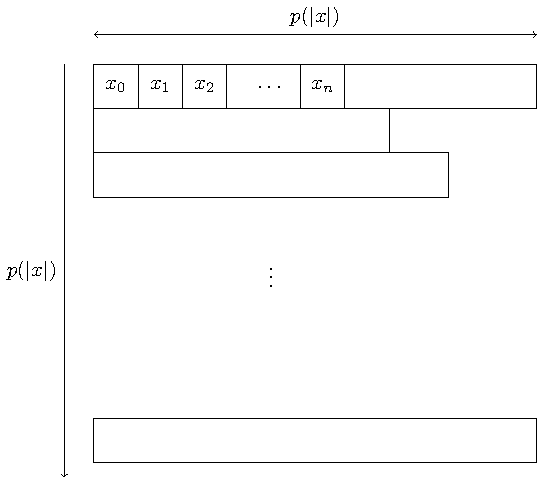
\includegraphics{./img/nondeterminism/SATproof1.pdf}
            \caption{Possiamo descrivere le possibili computazioni di una MdTN $M$ mediante una
            tabella cosi' fatta.}
        \end{center}
    \end{figure}

    Vogliamo descrivere questa matrice con una formula proposizionale. Questa matrice non e' unica,
    dato che esistono varie computazioni. La prima riga e' fissata alla configurazione iniziale, e
    l'ultima da quella finale. Lasciamo la liberta' alla matrice di rappresentare varie
    computazioni, dato che una riga non e' deterministicamente determinata da quella che la precede.

    %Slide 121

    Come rappresentiamo la matrice con una formula proposizionale?
    %Abbiamo a disposizione tutte le variabili che vogliamo.
    Usiamo delle variabili $y_{i,j,x}$. $i$ rappresenta il tempo (il passo $i$ della computazione),
    $j$ corrisponde alla cella, e $x$ al simbolo dell'alfabeto della matrice che sta nella cella $j$
    al tempo $i$.  La variabile e' vera se $x$ e' nella cella $j$ al tempo $i$, e falsa altrimenti.
    Vogliamo ora costruire un sistema di vincoli che corrisponde all'esistenza di una computazione
    accettante che utilizzi questo tipo di variabili. Per esprimere questi vincoli usiamo delle
    formule proposizionali.

    Definimao le ``cornici'' della matrice: prima e ultima configurazione, e i due lati della
    matrice. Possiamo supporre che il riconoscimento, se avviene, avvenga esattamente al momento
    $p(|x|)$. E' facile imporre questo vincolo anche su computazioni che accettano prima. L'alfabeto
    che stiamo considerando per questa matrice e' l'alfabeto $\Gamma' = \Gamma \cup (Q \times
    \Gamma)$, dove $\Gamma$ e' l'alfabeto di $M$ e la seconda parte codifica lo stato interno e la
    posizione della testina. Dove sta la coppia $q,x$ e' posizionata la testina. Inoltre abbiamo che
    lo stato interno e' $q$. Poiche' stiamo lavorando con un solo nastro ci aspettiamo che la
    testina sia su un solo carattere in ogni istante della computazione.

    Perche' vogliamo definire il bordo? Per semplicita'. E' abbastanza importante definirlo.
    %Supponiamo che $x = x_{1}\dotsc x_{n}$.
    Vogliamo che i bordi non siamo oltrepassati: li settiamo a blank e
    faremo in modo che rimangano blank per il resto della computazione.

    \begin{figure}[h]
        \begin{center}
            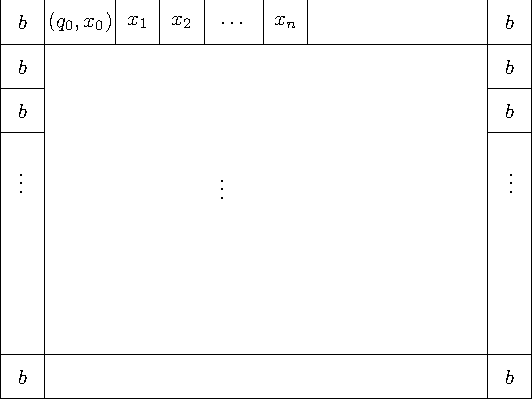
\includegraphics{./img/nondeterminism/SATproof2.pdf}
            \caption{Facciamo in modo che i bordi della tabella abbiano sempre il simbolo blank e
            che la prima riga corrisponda alla configurazione iniziale di $M$}
        \end{center}
    \end{figure}

    %Slide 122

    Possiamo iniziare a definire qualche vincolo. Vogliamo che ogni cella della matrice contenga uno ed
    un solo carattere. Questo vincolo e' espresso dalla seguente formula proposizionale:
    \begin{equation*}
        \phi_{0} = \bigwedge_{i=0}^{p(n)}\bigwedge_{j=0}^{p(n)}\left(\bigvee_{a \in \Gamma'}
            y_{i,j,a}
        \land \bigwedge_{a,b \in \Gamma',a \not= b}(\lnot y_{i,j,a} \lor \lnot y_{i,j,b})\right)
    \end{equation*}
    
    Per ogni istante di tempo da $i$ a $p(n)$, per ogni cella da $j$ a $p(n)$ almeno una delle
    variabili $y_{i,j,a}$ deve avere valore true. La dimensione della formula e' quadratica, ma per
    noi va bene perche' e' polinomiale. Vogliamo che tutte queste formule siano polinomiali in
    dimensione. La seconda parte del vincolo corrisponde a esprimere il fatto che vogliamo che una
    sola variabile abbia valore true tra le varie $y_{i,j,a}$ con $i$ e $j$ fissati.

    Questo vincolo e' un vincolo di ``soundness'' sulla matrice. Vogliamo ora esprimere il vincolo che
    sui bordi ci siano i caratteri blank. Questo e' espresso dalla seguente formula:
    \begin{equation*}
        \phi_{1} = \bigwedge_{i=0}^{p(n)}(y_{i,0,B} \land y_{i,p(n)+1,B})
    \end{equation*}

    Vogliamo fissare la configurazione iniziale e quella finale. Sappiamo com'e' fatta la configurazione
    iniziale, ed esprimiamo il vincolo che la matrice esprima quella configurazione nella prima riga con
    la seguente formula:
    \begin{equation*}
        \phi_{2} = y_{0,1,(q_{0},x_{0})} \land \bigwedge_{j=2}^{n}(y_{0,j,x_{j}}) \land
        \bigwedge_{j=n+1}^{p(n)}y_{i,j,B}
    \end{equation*}

    Ci aspettiamo che il carattere 0 sia $(q,x_{0})$, che nelle restanti celle ci siano i simboli
    dell'input, e che tutte le celle da $n$ in poi siano blank.

    Ci aspettiamo poi che l'ultima riga della matrice sia una configurazione di accettazione.
    Vogliamo ovvero che corrisponda ad una configurazione finale, ovvero che da qualche parte sul
    nastro la testina si sia arrestata in uno stato di accettazione. In termini della matrica ci
    aspettiamo che nell'ultima riga ci sia una cella con un carattere $F \times \Gamma$, dove $F$
    rappresenta il sottoinsieme di $Q$ di stati accettanti. Questo e' espresso dalla seguente
    formula:
    \begin{equation*}
        \phi_{3} = \bigvee_{j={1}}^{p(n)}\bigvee_{a \in F \times \Gamma}(y_{p(n),j,a})
    \end{equation*}

    Ci resta da descrivere la parte interna della matrice. In che modo vogliamo descrivere questa
    matrice? Come saranno fatte due righe successive? Saranno quasi identiche, dato che sono due
    configurazioni successive della computazione di $M$. Il nastro, durante un passo di
    computazione, cambia poco, dato che le operazioni tipiche di una MdT sono la scrittura di un
    carattere, lo spostamento della testina e il cambio del proprio stato interno. Supponiamo che la
    testina sia un una posizione $j$ con stato $q$ e carattere $a$. Cosa rimarra' sicuramente
    indentico nella riga successiva? Tutte le celle prima la cella $j-1$ e tutte le celle successive
    alla $j+1$. Al piu' cambiano 6 celle, in base alla riscrittura del carattere e al movimento
    della testina. 

    \begin{figure}[h]
        \begin{center}
            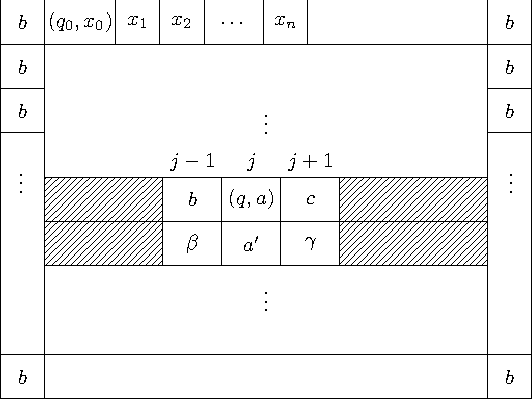
\includegraphics{./img/nondeterminism/SATproof3.pdf}
            \caption{Le uniche celle che cambiano durante un passo di computazione sono le 6 celle
                che comprendono quella con la testina e le altre 5 adiacenti. Avremo che $\beta = b$ e
                $\gamma = (q,c)$ se la testina si muove a destra, oppure $\beta = (q,b)$ e $\gamma = c$
            se la testina si muove a sinistra}
        \end{center}
    \end{figure}
    %Slide 123

    Esprimiamo questo con la seguente formula:
    \begin{equation*}
        \phi_{4} = \bigwedge_{i=0}^{p(n)-1}\bigwedge_{j=1}^{p(n)}\bigwedge_{a,b,c\in \Gamma}
        (y_{i,j-1,a} \land y_{i,j,b} \land y_{i,j+1,c} \implies y_{i+1,j,b})
    \end{equation*}
    Sappiamo che, se su una cella $j$ non c'e la testina e la testina non e' ne' nella cella $j-1$
    ne' in quella $j+1$ allora il carattere in $j$ non cambia.  Questo vale per tutte le celle.

    Finora non abbiamo usato molto della Macchina di Turing. Queste condizioni dipendenvano
    dall'alfabeto della macchina, dagli stati e dall'input. Quello che vogliamo ora esprimere
    dipende dalla funzione di transizione di $M$.

    La seguente formula richiede che per tutte le celle prima dell'ultima riga valga una certa
    formula $\Delta$, che andiamo a definire, e che dipende anche dai simboli di $Q \times F$:
    \begin{equation*}
        \phi_{5} = \bigwedge_{i=0}^{p(n)-1}\bigwedge_{j=1}^{p(n)}\bigwedge_{(q,a)\in Q\times F}
        \Delta_{q,a,i,j}
    \end{equation*}

    %Slide 124

    $\Delta_{q,a,i,j}$ e' una formula implicativa. Supponiamo che al tempo $i$ in posizione $j$ ci
    sia la testina ed un carattere $a$, ovvero supponiamo che $y_{i,j,(q,a)}$ sia vera. Supponiamo
    inoltre che siano vere $y_{i,j-1,b}$ e $y_{i,j+1,c}$. Cosa possiamo dire di come sara' fatto il
    nastro al prossimo passo? Dipende dal programma. Consideriamo un caso particolare. Supponiamo
    che, con stato $q$ e carattere $a$, la funzione di transizione abbia due possibilita':
    \begin{equation*}
        \delta(q,a) = \set{(q',a',R),(q'',a'',L)}
    \end{equation*}
    In generale potremmo avere un numero finito diverso di possibilita'. Supponiamo che la macchina non
    deterministica scelga la prima strada. Ci aspettiamo allora che $y_{i+1,j-1,b} \land y_{i+1,j,a'}
    \land y_{i+1,j+1,(q',c)}$. Questa' e' una possibilita'. Ci aspetteremmo quindi che valga questa oppure
    $y_{i+1,j-1,(q'',b)},y_{i+1,j,a''},y_{i+1,j+1,c}$. In generale ci aspettiamo un or tra le
    possibilita'. 
    %Nel caso generale avremo un or tra tutte le possibilita'. 
    La formula $\Delta$ nel caso generale e' cosi' fatta:
    \begin{align*}
        \Delta_{q,a,i,j} &= \bigwedge_{b,c \in \Gamma}( y_{i,j-1,b} \land y_{i,j,(q,a)} \land
        y_{i,j+1,c} \\ &\implies \bigvee_{(q',a',M) \in \delta(q,a)}(y_{i+1,j-1,\beta_{M,q',b}} \land
        y_{i+1,j,a'} \land y_{i+1,j+1,\gamma_{M,q',c}}))
    \end{align*}
    dove
    \begin{equation*}
        \beta_{M,q',b} =
        \begin{cases}
            \case{(q',b)}{se $M = L$}\\
            \case{b}{altrimenti}\\
        \end{cases}
    \end{equation*}
    e
    \begin{equation*}
        \gamma_{M,q',c} =
        \begin{cases}
            \case{(q',c)}{se $M = R$}\\
            \case{c}{altrimenti}\\
        \end{cases}
    \end{equation*}

    Se c'e' una computazione accettante la formula $\phi_{x}^{M,p} = \phi_{0} \land \phi_{1} \land
    \phi_{2} \land \phi_{3} \land \phi_{4} \land \phi_{5}$ e' soddisfacibile. Viceversa se questa
    formula e' soddisfacibile allora $M$ era in grado di seguire una computazione che l'avrebbe
    portata al riconoscimento della stringa. Di conseguenza abbiamo che $A \leq_{p} SAT$. L'unico
    vincolo che abbiamo sul numero e sulla dimensione delle formule e' un vincolo di tipo
    polinomiale. Questa condizione e' pero' facilmente verificata. Questo conclude la dimostrazione.

\end{proof}

Con le formule proposizionali riusciamo a descrivere una cosa complessa come una computazione di una
MdTN. In generale con formule proposizionali possiamo esprimere e modellare molte cose, da cui le
tante riduzioni a $\SAT$ o $3\SAT$.

Quando abbiamo un problema $B$ $\NPClass$-completo e' interessante aggiungere vincoli per capire se
$B$ rimane $\NPClass$-completo. Ad esempio abbiamo visto che la 3-colorabilita' e'
$\NPClass$-completo, mentre la 2-colorabilita' e' in $\PClass$. A volte riusciamo ad aggiungere
abbastanza vincoli da restringerci da un problema $\NPClass$-completo ad un prolema in $\PClass$.

Sappiamo che le formule proposizionali possono essere espresse in delle forme normali. Le forme
normali tipiche sono la congiuntiva e disgiuntiva.  Una formula e' in forma normale congiuntiva
(Conjunctive normal form, CNF) se puo' essere espressa come una congiunzione di clausole, dove la
clausole sono disgiunzioni di letterali. Un letterale e' una variabile proposizionale o la sua
negata. Possiamo esprimere una clausola $A \land \lnot A \land C$ con una notazione insiemistica
come $\set{A,\lnot A,C}$. Questo perche' l'or e' idempotente: $A \lor A \equiv A$. Possiamo inoltre
rappresentare una conginzione di congiunzioni con una notazione insiemistica come ad esempio
$\set{\set{A,\lnot A,C},\set{A,\lnot B}}$.

Che vincoli possiamo immaginare di porre a $\SAT$? Possiamo immaginare di dare un vincolo al numero
di letterali nelle clausole. Se poniamo un vincolo di 3 letterali in ogni clausola otteniamo
$3\SAT$, l'insieme delle formule soddisfacibili espresse in CNF con clausole di 3 letterali.

Otteniamo in questo modo un problema piu' semplice di $\SAT$? Vedremo che in realta' no, poiche'
$\SAT \leq 3\SAT$.

\section{Riduzioni di problemi $\NPClass$-completi}

\subsection{$\SAT \leq 3\SAT$}

%Siamo ora interessati ad una ``restrizione'' di $\SAT$: $3\SAT$.

\begin{thm}
        $\SAT \leq 3\SAT$.
\end{thm}

Mostriamo ora che $3\SAT$ e' $\NPClass$-completo mostrando una riduzione da $\SAT$ a $3\SAT$. Per
fare cio' ci serve una trasformazione che richiede tempo polinomiale da formule generali a formule
in 3-CNF tale che conservi la soddisfacibilita' della formula.

Quando vogliamo facciamo una trasformazione di una formula di solito vogliamo ottenere una formula
equivalente a quella di partenza. In questo caso a noi interessa una cosa piu' debole: ottenere una
formula che sia soddisfacibile sse la formula di partenza era soddisfacibile.

Vediamo perche' non ci conviene usare una trasformazione che ci permtte di passare ad una formula
logicamente equivalente a quella di partenza. Data una qualsiasi formula della logica proposizionale
possiamo trasformarla in una logicamente equivalente in forma normale congiuntiva. Possiamo fare
questo perche' esistono varie equivalenze logiche notevoli che ci permettono di dare alla formula la
forma che desideriamo: ad esempio, $A \implies B \equiv \lnot A \lor B$.

Il primo passaggio e' trasformare tutti i connettivi nelle formule in loro corrispettivi equivalenti
espressi con $\lor,\land,\lnot$. Dopodiche' ``pushiamo'' le negazioni al piu' interno possibile nella
formula. Le regole che ci permettono di propagare la negazione all'interno della formula sono le
formule di de Morgan: ad esempio $\lnot (A \land B) \equiv \lnot A \lor \lnot B$. La propagazione
della negazione si blocca quando giungiamo alle formule atomiche. Abbiamo ancora un nesting
arbitrario di congiunzioni e disgiunzioni pero'. Questo puo' essere risolto utilizzando le regole di
distributivita': ad esempio, $A \lor (B \land C) \equiv (A \lor B) \land (A \lor C)$.

In questo modo possiamo ottenere una formula equivalente in 3-CNF. Abbiamo pero' un problema
abbastanza grave: in generale questa trasformazione puo' portare ad una esplosione esponenziale
della dimensione della formula. Questa trasformazione richiede quindi tempo esponenziale, e di
conseguenza non si tratta di una riduzione polinomiale.

Noi pero' siamo interessati alla soddisfacibilita'. Se non siamo interessati a preservare
l'equivalenza logica possiamo usare una trasformazione che conserva la soddisfacibilita' e che non
porta ad un'esplosione esponenziale.

Vediamo questa trasformazione con un esempio. Prendiamo la formula seguente:
\begin{equation}\label{eq:start}
    \bigwedge_{i=1}^{n}(x_{i}\land y_{i}) = (x_{1} \land y_{1}) \land \cdots \land (x_{n} \land y_{n})
\end{equation}

Se la trasformassimo in una formula equivalente utilizzando il metodo appena descritto otterremmo le
$2^{n}$ clausole:
\begin{equation*}
    \set{x_{1},\dotsc,x_{n-1},x_{n}},\set{x_{1},\dotsc,x_{n-1},y_{1}},\dotsc,\set{y_{1},\dotsc,y_{n-1},y_{n}}
\end{equation*}

Se invece passiamo dalla formula di partenza alla seguente, espressa come insieme di clausole:
\begin{equation}\label{eq:transformation}
    \set{z_{1},\dotsc,z_{n}},\set{\lnot z_{1},x_{1}},\set{\lnot z_{1},y_{1}},\dotsc,\set{\lnot
    z_{n},x_{n}},\set{\lnot z_{n},y_{n}}
\end{equation}
Otteniamo una formula soddisfacibile se e solo se lo era quella di partenza, ma che non e' ad essa
logicamente equivalente.  Inoltre la dimensione aumenta in modo lineare.  Ogni $z_{i}$ ci indica se
la coppia $x_{i} \land y_{i}$ era vera.

Se introduciamo variabili diverse due formule non possono essere equivalenti. Le equivalenze si
stabbiliscono tra formule con le stesse variabili.

Se la formula \ref{eq:transformation} e' vera almeno uno $z_{i}$ deve essere vero. In piu' tutte le
altre clausole devono essere vere. Dove $z_{i}$ e' vero sia $x_{i}$ che $y_{i}$ devono essere veri.
Ma allora era vera anche la formula \ref{eq:start}.

Adottando questa tecnica e' possibile dimostrare che ogni formula proposizionale puo' essere
trasformata in 3-CNF preservando la soddisfacibilita' con una crescita' al piu' polinomiale.

In generale non e' vero che possiamo trasformare una formula in una equivalente in CNF in tempo
polinomiale. Se siamo interessati alla soddisfacibilita' possiamo fare una trasformazione
polinomiale che ci restituisce una formula ``soddsifacibilmente equivalente'' a quella di partenza.
In particolare quest'ultima trasformazione non preserva la tautologicita' di una formula.

\subsection{$3\SAT \leq \VC$}

Vediamo ora un teorema abbastanza importante. E' un esempio interessante di riduzione. Vogliamo
dimostrare che $3\SAT$ e' riducibile a $\VC$.

\begin{thm}
        $3\SAT \leq \VC$
\end{thm}

Ricordiamo che $\VC$ e' il problema del ricoprimento di vertici:
\begin{equation*}
    \VC = \set{\pair{G}{k} \mid \text{Esiste un ricoprimento di vertici in $G$ di dimensione $\leq k$}}
\end{equation*}

Un ricoprimento di vertici e' un sottoinsieme $S$ di $V$ tale che per ogni arco uno dei nodi
dell'arco ricade in $S$.

Sono due problemi a priori diversi. Ci si potrebbe chiedere cosa abbia a che fare l'uno con l'altro.
Le riduzioni, in genere, mettono in relazione mondi diversi: ci permettono di vedere vari problemi
in modi diversi ma equivalenti.

La prima cosa da chiedersi quando si vuole fare una riduzione e' cosa richiedono in input il primo e
il secondo problema. $3\SAT$ richiede una formula $\varphi$ in 3-CNF e decide se questa e'
soddisfacibile o meno. Vertex Cover prende in input un grafo $G$ ed un intero $k$. La $f$ che
vogliamo costruire prende in input la formula $\varphi$ e restituisce in output una coppia
$\pair{G}{k}$. Inoltre vogliamo che $f \in \FP$.
\begin{equation*}
    \varphi \overset{f}{\mapsto} \pair{G}{k}
\end{equation*}

Dobbiamo inoltre dimostrare che $\varphi \in 3\SAT \iff \pair{G}{k} \in \VC$. La definizione di $f$
richiede del lavoro creativo.

Partiamo da un esempio. Supponiamo di avere una formula cosi' fatta:
\begin{equation*}
    \phi = \set{\set{A,\lnot B, C},\set{\lnot A, B \lnot C},\set{\lnot A,\lnot B, C},\set{A,B,\lnot
    C}}
\end{equation*}

Questa formula e' soddisfacibile. Se prendessimo la congiunzione di tutte le 8 possibili clausole la
formula sarebbe insoddisfacibile. E' facile verificare che qualsiasi sottoinsieme stretto delle
possibili clausole sarebbe soddisfacibile. Questo ci mostra che nonostante $3\SAT$ sia un problema
$\NPClass$-completo possono esistere delle euristiche che ci aiutano a capire se una formula e'
soddisfacibile o meno in maniera efficiente per certi casi particolari.

Da questa formula dobbiamo ottenere un grafo ed assegnargli un $k$. Il grafo $G$ e' fatto cosi':
\begin{itemize}
        \item Colleghiamo con un arco ogni letterale con il suo negato, creando un insieme di coppie
        \item Creiamo dei ``triangoli'' per ogni clausola
        \item Collegiamo i letterali tra di loro tra le coppie e i triangoli
\end{itemize}
La costruzione e' rappresentata nelle figure \ref{img:SATtoVC1} e \ref{img:SATtoVC2}

\begin{figure}[h]
    \begin{center}
        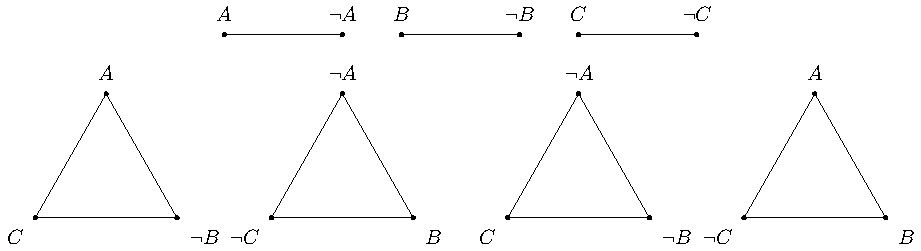
\includegraphics[scale=0.75]{./img/nondeterminism/SATtoVC1.pdf}
        \caption{Strutture di base del grafo $G$: coppie e triangoli}
        \label{img:SATtoVC1}
    \end{center}
\end{figure}

\begin{figure}[h]
    \begin{center}
        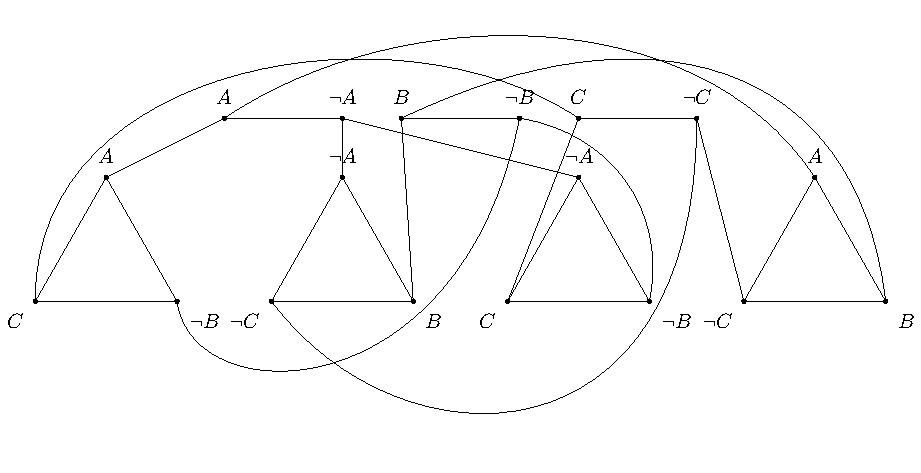
\includegraphics[scale=0.75]{./img/nondeterminism/SATtoVC2.pdf}
        \caption{Aggiunta degli archi tra i vertici del grafo}
        \label{img:SATtoVC2}
    \end{center}
\end{figure}

Quanti sono i nodi del grafo? Supponiamo che $n$ sia il numero delle variabili ed $m$ il numero
delle clausole. Per il nostro esempio $n=3$ e $m=4$. Abbiamo che il numero di nodi e' $2n + 3m$.

E' un grafo abbastanza sparso. Potremmo contare gli archi, ma e' abbastanza evidente che questi
siano in numero lineare nel numero dei nodi.

Quanti nodi dobbiamo prendere per coprire tutti gli archi? Per i triangoli almeno 2; per le coppie
almeno 1. Un ricoprimento deve avere una dimensione minima $2m + n$. Questo sara' il nostro $k$
della riduzione. Abbiamo quindi la nostra trasformazione $f$. Vogliamo dimostrare che se questo
grafo ha un ricoprimento di cardinalita' $\leq k$ la formula di partenza e' soddisfacibile, e
viceversa.

Mostriamo i due versi del sse, che sono abbastanza diversi.

Supponiamo che $\varphi$ sia soddisfacibile. Esiste quindi un'assegnamento di valori di verita' che
rende la formula soddisfacibile. Nel nostro esempio andrebbe bene l'assegnamento che assegna falso a
tutte le variabili proposizionali. Nel nostro grafo nelle coppie scegliamo per il ricoprimento il
letterale che, in base all'assegnemento, ha valore vero. In questo caso prenderemmo $\lnot A, \lnot
B, \lnot C$. Nei triangoli delle clausole abbiamo che c'e' un letterale direttamente collegato ad
uno dei letterali gia' scelti. Ad esempio, nel primo triangolo abbiamo che $\lnot B$ e' collegato al
corrispondente nella seconda coppia. Questo arco tra i due $\lnot B$ e' gia coperto. Di conseguenza
scegliamo per il ricoprimento gli altri due nodi. Facciamo questo per ogni clasuola. Quello che
otteniamo e' un ricoprimento su $G$ di dimensione $2m + n$. Quindi se $\varphi$ e' soddisfacibile
esiste un ricoprimento di dimensione $\leq k$.

Prendiamo ora il verso opposto. Supponiamo esista un ricoprimento di dimensione $2m + n$. Se abbiamo
un tale ricoprimento abbiamo che per ogni triangolo abbiamo preso almeno due vertici e per ogni
coppia abbiamo preso uno dei vertici. Per l'assegnamento dei valori di verita' assegnamo valore vero
ai vertici presi dalle coppie. Abbiamo che uno dei nodi, per ogni triangolo, deve toccare uno dei
nodi che abbiamo selezionato nelle coppie. Di conseguenza tale assegnamento di valori di verita'
soddisfa la formula. Di conseguenza se esiste un ricoprimento di dimensione $2m + n$ abbiamo che la
$\varphi$ corrispondente e' soddisfacibile.

\begin{figure}[h]
    \begin{center}
        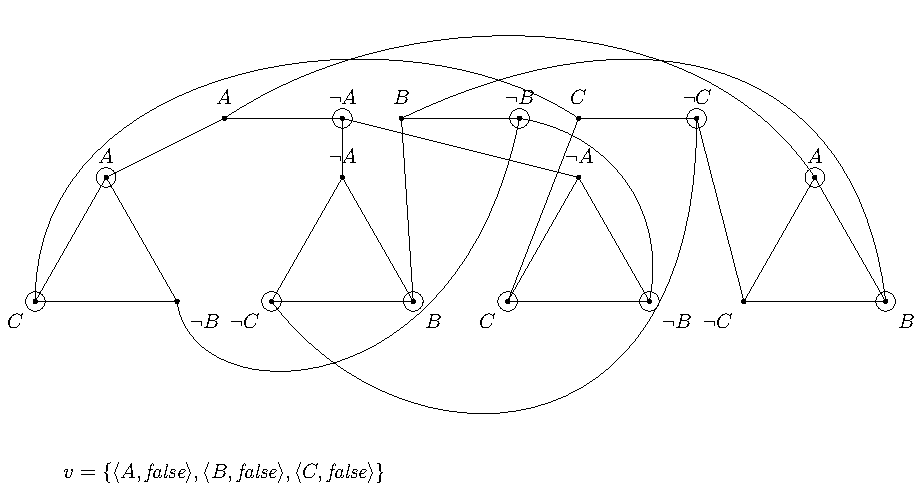
\includegraphics[scale=0.75]{./img/nondeterminism/SATtoVC3.pdf}
        \caption{I nodi cerchiati nel grafo $G$ fanno parte del sottoinsieme $S$ di copertura dei
        vertici}
    \end{center}
\end{figure}

Questo ci mostra, nuovamente, quanto siano importanti i grafi in informatica: sono una struttura
dati flessibile che ci permette di modellare molti problemi. Molti di questi possono essere espressi
come problemi di visita su grafi.

Abbiamo gia' visto che $\VC$ e' equivalente al problema della cricca e al problema dell'insieme
indipendente. Di conseguenza, poiche' abbiamo che $\VC$ e' $\NPClass$-completo per la dimostrazione
appena vista, abbiamo che anche cricca e insieme indipendente sono problemi $\NPClass$-completi.

\subsection{$\HAMPATH \equiv \HAMCYCLE$}

Vediamo una riduzione dal problema del cammino hamiltoniamo al ciclo hamiltoniano e una riduzione
inversa. Questi due problemi sono equivalenti.

Quello che vogliamo per ridurre il cammino hamiltioniano al ciclo hamiltoniano e' una riduzione tra
grafi che ci porti dal problema dell'esistenza di un cammino hamiltioniano al problema
dell'esistenza di un ciclo hamiltoniano.

Quello che facciamo e' aggiungere un nodo collegato a tutti i nodi del grafo $G$ di partenza.

\begin{figure}[h]
    \begin{center}
        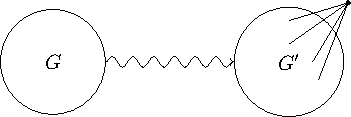
\includegraphics{./img/nondeterminism/HAMPATHCYCLE.pdf}
        \caption{Aggiungendo un nodo collegato a tutti gli altri trasformiamo un qualsiasi cammino
        hamiltoniano esistente in $G$ in un circuito che passa per il nuovo nodo}
    \end{center}
\end{figure}

Se abbiamo un cammino hamiltoniano in $G$ otteniamo un ciclo in $G'$ passando per il nuovo nuovo $n$
aggiunto dall'ultimo nodo del cammino e passando al primo nodo del cammino. Viceversa, se abbiamo un
ciclo in $G'$ questo include necessariamente $n$. Togliendo $n$ dal ciclo otteniamo un cammino
hamiltoniano in $G$.

L'altro verso e' piu' complesso. Non basta l'identita' come trasformazione perche' con questa non
vale il sse. L'identita' serve in genere a ridurre un problema a se stesso.

L'idea e' la seguente: partendo dal grafo selezioniamo un nodo arbitrario $n$. Questo nodo avra' un
po' di connessioni con altri nodi. Costruiamo una copia di questo nodo: aggiungiamo un nodo nuovo
$n'$ collegato a tutti i nodi a cui era collegato $n$. Aggiungiamo poi due nuovi nodi $m,m'$
collegati, rispettivamente, a $n$ e $n'$.

Il grafo $G'$ cosi' costruito a partire da $G$ ha un cammino hamiltoniano sse $G$ aveva un ciclo
hamiltoniano. Infatti sia $n$ il nodo che viene ``clonato'' in $G$ e sia $p = n_{1}, \dotsc,
n_{i-1}, n, n_{i}, \dotsc, n_{n}, n_{1}$ un ciclo hamiltoniano in $G$. In $G'$ costruiamo un cammino
hamiltoniano a partire da $p$ nel seguente modo: partiamo da $m$, passiamo per $n$, e seguiamo $p$
in un qualche verso. Ad esempio da $n$ passiamo a $n_{i}$ fino a tornare a $n_{i-1}$. A questo punto
da $n_{i-1}$ passiamo al nodo clone $n'$ e da li' passiamo infine ad $m'$. Possiamo passare da
$n_{i-1}$ a $n'$ poiche' $n'$ e' collegato a tutti i nodi adiacenti ad $n$, e $n_{i-1}$ e' adiacente
ad $n$.

Viceversa, se in $G'$ abbiamo un cammino hamiltoniano allora abbiamo un circuito hamiltoniano in
$G$. Infatti se esiste un cammino hamiltoniano $p'$ questo deve necessariamente avere come estremi
del cammino $m$ e $m'$. Sia, ad esempio, $p' = m, n, n_{i},\dotsc, n_{i-1}, n', m'$. Da $p'$
possiamo ottenere un ciclo hamiltoniano in $G$ nel seguente modo: da $p'$ rimuoviamo $m, n'$ e $m'$
e aggiungiamo $n$ in fondo per chiudere il circuito. Siamo sicuri che questo sia un circuito
hamiltoniano in $G$ poiche' se $n_{i-1}$ era adiacente a $n'$ allora necessariamente era adiacente
anche ad $n$.

Illustriamo questa trasformazione con l'esempio in figura \ref{img:HAMCYCLEPATH}.

\begin{figure}[h]
    \begin{center}
        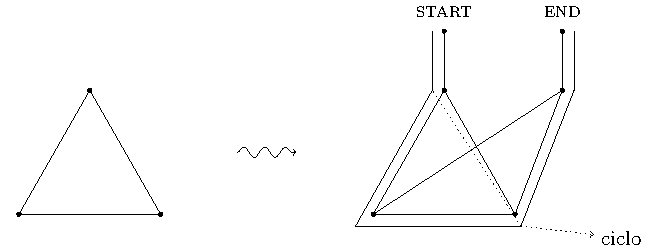
\includegraphics{./img/nondeterminism/HAMCYCLEPATH.pdf}
        \caption{Da un ciclo hamiltoniano in $G$ passiamo ad un cammino hamiltoniano in $G'$ e,
        viceversa, da un cammino hamiltoniano in $G'$ passiamo ad un ciclo in $G$}
        \label{img:HAMCYCLEPATH}
    \end{center}
\end{figure}

%Esercizio per la prossima volta. Prendiamo il problema del cammino ed il problema del cammino
%puntato. Il problema del cammino prende un grafo. Il problema del cammino puntato prende un grafo e
%due nodi. Il primo cerca di capire se esiste un cammino hamiltoniano. Il secondo cerca di capire se
%esiste un cammino hamiltoniano che parte dal primo nodo al secondo. Quest'ultimo semrerebbe piu'
%semplice. In realta' rimane NP-completo. Dimostrare una riduzione da CAM a CAM PUNTATO.
